\documentclass[manuscript]{aastex62}

\usepackage{bm}
\usepackage{amsmath}
\usepackage{color}
\usepackage{comment}
\usepackage{graphicx}
%\usepackage{minted}


\received{\today}
\revised{\today}
\accepted{\today}

% scaffolding
\definecolor{cerulean}{HTML}{2a52be}
\newcommand{\todo}[1]{\textcolor{cerulean}{#1}}

% stellar things
\newcommand\teff{T_{\rm eff}}
\newcommand\logg{\log{g}}
\newcommand\feh{[\rm{Fe}/\rm{H}]}
\newcommand\mh{[\rm{M}/\rm{H}]}
\newcommand{\luminosity}{L_\circ}
\newcommand{\radius}{R_\circ}

% maaaaath 
\newcommand{\vect}[1]{\boldsymbol{\mathbf{#1}}}
\renewcommand{\vec}[1]{\vect{#1}}
\newcommand{\vectheta}{\vec{\theta}}
\newcommand{\likelihood}{\mathcal{L}}
\newcommand{\given}{|}
\newcommand{\transpose}{^\textrm{T}}


% projects
\newcommand{\project}[1]{\textsl{#1}}
\newcommand{\package}[1]{\texttt{#1}}
\newcommand{\acronym}[1]{{\small{#1}}}
\newcommand{\ESA}{\acronym{ESA}}
\newcommand{\Gaia}{\project{Gaia}}
\newcommand{\gaia}{\project{gaia}}
\newcommand{\Grp}{\textrm{G}_\textrm{RP}}
\newcommand{\Gbp}{\textrm{G}_\textrm{BP}}
\newcommand{\G}{\textrm{G}}
\newcommand{\MG}{M_\textrm{G}}
\newcommand{\MGRP}{M_{\textrm{G}_{\textrm{RP}}}}
\newcommand{\MGBP}{M_{\textrm{G}_{\textrm{BP}}}}

\newcommand{\foreign}[1]{\emph{#1}}
\newcommand\ie{\foreign{i.e.}}
\newcommand\eg{\foreign{e.g.}}

% definitions
\newcommand{\GaiaRVE}{\sigma_{\mathrm{V}_\mathrm{R}}^\mathrm{MTA}}
%\newcommand{\RVJitter}{\sigma(\mathrm{V}_\mathrm{R}^{t})}
\newcommand{\RVJitter}{j_{rv}}
\newcommand{\AstJitter}{j_{a}}

% for version control
\newcommand{\vcpath}{vc.tex}

% for figures
\newcommand{\CheckSum}{rc.4}


\graphicspath{{../results/\CheckSum/figures/}}


\IfFileExists{\vcpath}{\input{\vcpath}}{
	\newcommand{\giturl}{UNKNOWN}
	\newcommand{\gitslug}{UNKNOWN}
	\newcommand{\githash}{UNKNOWN}
	\newcommand{\gitdate}{UNKNOWN}
	\newcommand{\gitauthor}{UNKNOWN}
	\newcommand{\watermarktext}{DRAFT}
}

\submitjournal{AAS}

\shorttitle{Stellar multiplicity in the second \Gaia\ data release}
\shortauthors{Casey et al.}

\begin{document}

\title{Stellar multiplicity in the second \Gaia\ data release}

\correspondingauthor{Andrew R. Casey}
\email{andrew.casey@monash.edu}


\author[0000-0003-0174-0564]{Andrew R. Casey}
\affiliation{School of Physics \& Astronomy, 
			 Monash University,
			 Wellington Rd, Clayton 3800, Victoria, Australia}

\author[0000-0002-9328-5652]{Daniel Foreman-Mackey}
\affiliation{Flatiron Institute, 
			 162 Fifth Ave, New York, NY 10010, USA}

\author[0000-0003-3494-343X]{Carles Badenes}
\affiliation{Department of Physics and Astronomy, 
			 University of Pittsburgh, 
			 3941 O'Hara Street, Pittsburgh, PA 15260, USA}

\author[0000-0003-0872-7098]{Adrian Price-Whelan}
\affiliation{Flatiron Institute, 
			 162 Fifth Ave, New York, NY 10010, USA}

% Others to thank and/or invite to contribute:
% David Hogg
% Hans-Walter Rix
% Kareem El-Badry
% Daniel Michalik
% Rosemary Mardling


\begin{abstract}
The frequency and properties of unresolved stellar companions underpins much of astrophysics.
These systems are challenging to detect and characterise.
% as their sensitivity depends on both the properties of the orbit and the system orbital and source properties.
Here we self-calibrate the noise in astrometric and radial velocity measurements in the second 
\Gaia\ data release, and we use excess noise to detect and partially characterise binary systems.
%Given a \Gaia\ radial velocity error, we detect binaries with orbital periods $P \lesssim 1,300\,{\rm days}$ and semi-amplitudes $K_1 \gtrsim 1\,{\rm km\,s}^{-1}$. 
%Using astrometric noise we reliably detect unequal mass binary star systems out to \todo{X}\,pc with \todo{Y\%} completeness.
After simulating what \Gaia\ would observe and accounting for systematics and detection efficiencies, 
we find that \todo{$X^{+Y}_{-Z}$}\% \Gaia\ sources have one or more unresolved stellar companions. 
We find the frequency of stellar multiples increases at low metallicities, consistent with \todo{high redshift stuff.} 
For each source we provide probability estimates of that source being a single star, and estimates 
of orbital elements for systems that are likely to be stellar multiples.
\todo{Some comment on superlative systems.}
\end{abstract}

\keywords{Binary stars}


\section{Introduction} \label{sec:introduction}

\todo{
	\begin{itemize}
		\item Binarity affects many fields of astrophysics.
		\item Population inference necessary because it is difficult to infer multiplicity for a given source
		\item Many different methods available for individual sources, sensitive in different ways.
		\item Eventually \Gaia\ will solve all.
		\item Here we use noise in \Gaia\ to infer multiplicity.
	\end{itemize}
}
%In this work we make use of astrometry (including radial motion)
%from the second \Gaia\ data release to infer the presence of stellar companions 
%for millions of point sources.
%We provide partial characterisations of these systems,
%based on the data available for each source. In Section \ref{sec:method} we 
%describe our methods, and in Section \ref{sec:results} we outline our results 
%in context of other stellar multiplicity surveys. We include comparisons of 
%binary properties between clusters and the field, as a function of stellar 
%properties (e.g., stellar metallicity), and highlight some particularly 
%noteworthy systems that would benefit from additional observations. 


\section{Methods} \label{sec:methods}

Stellar multiplicity can be inferred from \Gaia\ data using radial velocity measurements, astrometry,
and/or photometry. These data are sensitive to stellar multiplicity in different ways. In the next 
sub-section we describe our methods for detecting stellar multiplicity from astrometric noise, 
before describing how our methods vary for radial velocities.
Here we do not directly use photometric variability to identify stellar multiples.
%despite the clear population of main-sequence binaries present in the 
%\Gaia\ data \citep{Lindegren:2018}. 
In later sections we show that these binary systems are identifiable by their 
jitter\footnote{Throughout this work when we use the term \emph{jitter} we are
	referring to the intrinsic uncertainty in measuring either the astrometric position or the radial 
	velocity.} in astrometry and/or radial velocity, and omitting photometric information avoids 
confusion with single stars that are photometrically variable.


\subsection{Astrometry} \label{sec:methods/astrometry}

We restrict our work to the brightest 16,676,756 sources in \Gaia\ DR2 \citep{Lindegren:2018}. 
\Gaia\ estimates the astrometric position of each source by measuring the photocenter in the G-band. 
If the source is a binary system with a mass ratio $q \neq 1$ then the photocenter changes as a 
function of the orbital parameters, as well as the system's parallax and proper motion.\footnote{The
	photocenter does not change for binary systems of equal mass and luminosities.} 
The uncertainty in astrometric position that is caused by orbital motion will remain after 
accounting for the apparent motion due to parallax and transverse velocity.


There are many sources of astrometric jitter for a given source, but here we will assume that the 
principal source of excess jitter is the presence of a stellar-mass companion. 
We take the reduced unit weight error (RUWE) as the measure of astrometric jitter
\begin{eqnarray}
	\AstJitter = \textrm{RUWE} = \sqrt{\frac{\chi^2_{al}}{N_{obs,al} - 5}} \label{eq:astrometric_unit_weight_error}
	\label{eq:define-ast-jitter}
\end{eqnarray}
\noindent{}where $\chi^2_{al}$ is the astrometric $\chi^2$ value in the along-scan direction (column
\texttt{astrometric\_chi2\_al}) and $N_{obs,al}$ is the number of astrometric observations in the 
along-scan direction (column \texttt{astrometric\_n\_obs\_al}). 
The RUWE is unaffected by the `degree of freedom bug' that occurred during the processing of the
second \Gaia\ data release \citep[e.g., see Appendix A1 of ][]{Lindegren:2018}, which resulted in
80\% of sources having no reported astrometric excess noise. 
The RUWE can be interpreted similarly to how the astrometric excess noise would be interpreted in 
that large values are less consistent with a single star model, but this must be considered in 
context with sources of similar colours, apparent G-band magnitudes, and to a lesser extent, 
absolute G-band magnitudes.

For these reasons we will assume that for a sample of sources of \emph{similar}
	$\Gbp\ - \Grp$ colour,
	apparent G-band magnitude $\G$, and
	absolute G-band magnitude $\MG$,
the distribution of astrometric jitter is a mixture of two components:
\begin{enumerate}
\item \emph{single-star systems},\\where the jitter represents the minimum uncertainty
	   with which \Gaia\ can measure the astrometric position for a source with those 
	   properties, and
      
\item \emph{stellar multiples},\\where the jitter is significantly higher 
	  than what is measured for single-star systems of similar properties.
\end{enumerate}

The latter component will include binary systems, trinaries, and other higher-order multiples. 
For practical purposes here we will assume that all stellar multiples are binary systems and will
(incorrectly) use the terms \emph{stellar multiples} and \emph{binaries} interchangeably.

We can expect that single stars should have a RUWE near 1 because it is a reduced $\chi^2$ 
distribution, but the expectation and variance of the RUWE will vary as a function of colour and 
magnitude. 
We cannot \emph{a priori} write down a relationship to describe how the expectation and variance 
of the RUWE will behave given some source properties because it is a complex function of unknown 
systematics.
For these reasons we adopt a non-parametric model for the astrometric jitter for single stars.

%Here we describe that model.
Consider a \Gaia\ source of interest. For this source we randomly draw at least 128 comparison 
sources (up to 1,024) that have a similar $\Gbp\ - \Grp$ colour (within $0.05\,\textrm{mag}$), 
and apparent and absolute G-band magnitudes that are both within $0.5\,\textrm{mag}$ of the source 
of interest.
Although we do not know yet which sources are single stars, we can assume that any single stars 
within this `ball' of parameter space should have comparable astrometric jitter. 
We will also assume that the randomly selected sample contains \emph{some} single stars, and 
\emph{some} stellar multiples. 
We do not care which is which. Here we are most interested in estimating the expected
jitter for single stars, and to do so we need to know what the jitter looks like for
single stars \emph{and} stellar multiples, otherwise we would under-estimate the typical astrometric
jitter for single stars.



In Figure~\ref{fig:example-mixture-model} we show the astrometric and radial velocity jitter 
(Eq \todo{X}) for a \Gaia\ source of interest and a comparison sample of sources with similar 
colours and magnitudes.
The distributions are clearly asymmetric, which we will fit with a two-component mixture model.
The first component is a normal (Gaussian) distribution to describe the jitter of single stars, 
and the second is a log-normal distribution to account for stellar multiples.
However, a log-normal distribution has sufficient flexibility to fit the entire distribution
(forcing the weight of the single star component to zero), so the avoid this we define the mean of
the log-normal distribution $\mu_m$ as
\begin{eqnarray}
	\mu_m \equiv \ln(\mu_s + \sigma_s) + \sigma_m^2
	\label{eq:mu_m}
\end{eqnarray}
\noindent{}where $\mu_s$ and $\sigma_s$ are the mean and standard deviation of the normal (single 
star) component and $\sigma_m$ is the standard deviation of the log-normal (stellar multiple)
component.
The $s$-subscript here refers to single stars, and $m$ for multiple. 
Fixing $\mu_m$ as per Equation \ref{eq:mu_m} forces the \emph{mode} of the log-normal distribution 
to be at $\mu_s + \sigma_s$, ensuring that the normal distribution is capturing the jitter of
single stars and the log-normal is capturing the extended tail of stellar multiples.
We experimented with different priors and model parameterisations and found that fixing $\mu_m$ had 
little to no effect on our inferences. The parameters of this two-component model are therefore $\vec\phi = \{w,\mu_s,\sigma_s,\sigma_m\}$ 
where $w$ is the mixing proportion. 


Initially we adopted uninformative priors on all parameters with physically motivated boundaries.
However, after performing prior predictive checks across the parameter space, we found two types of
model inconsistencies. 
The first occurred at low $\AstJitter$ values when the single star model had weak support 
(\eg, $w \lesssim \frac{1}{2}$ or $\sigma_s \ll \mu_s$).
The mode of the log-normal would remain at $\mu_s + \sigma_s$ by definition, but at low $\AstJitter$
values the log-normal component would have more probability support than the normal component.
In other words, certain combinations of $\vec\phi$ would mean that a source would be described as a
stellar multiple even if the $\AstJitter$ were very low.
The second inconsistency was similar in nature, where for certain combinations of $\vec\phi$ we 
observed the normal component to have higher probability than the log-normal component at high
values of $\AstJitter$ (\ie, $p_s > p_m$ at $\AstJitter \gg \mu_s + \sigma_s$). 
For these reasons we adopted the following priors,
\begin{eqnarray}
	w 			& \,\,\sim\,\, &	\mathcal{U}\left(\frac{1}{2}, 1\right) \\
	\mu_s 		& \,\,\sim\,\, & 	\mathcal{U}\left(\frac{1}{2}, 25\right) \\
	\sigma_s	& \,\,\sim\,\, & 	\mathcal{U}\left(\frac{1}{8}\mu_s, 5\right) \\
	\sigma_m 	& \,\,\sim\,\, & 	\mathcal{U}\left(\frac{\sigma_s}{\mu_s + \sigma_s}, 1\right)
\end{eqnarray}
\noindent{}and introduced a sigmoid function to penalise the log-normal probability at jitter values
$\AstJitter < \mu_s$. The likelihood is
\begin{eqnarray}
%	\mathcal{L}\left(\vec\phi\given\AstJitter\right) &\propto& \prod_{n=1}^{N} \left[\frac{w}{\sqrt{2\pi\sigma_s}}\exp\left(-\frac{[\AstJitter - \mu_s]^2}{2\sigma_s^2}\right) + \frac{1-w}{\AstJitter\sigma_m\sqrt{2\pi}}\exp\left(-\frac{(\ln\AstJitter - \mu_m)^2}{2\sigma_m^2}\right)\right] \\
	\mathcal{L}\left(\vec\phi\given\AstJitter\right) &\propto& \prod_{n=1}^{N} \left[\frac{w}{\sqrt{2\pi\sigma_s}}\exp\left(-\frac{[\AstJitter - \mu_s]^2}{2\sigma_s^2}\right) + \mathcal{S}\left(\AstJitter\right)\frac{1-w}{\AstJitter\sigma_m\sqrt{2\pi}}\exp\left(-\frac{(\ln\AstJitter - \mu_m)^2}{2\sigma_m^2}\right)\right]
\end{eqnarray}
\noindent{}where the sigmoid $\mathcal{S}\left(\AstJitter\right)$ is
\begin{eqnarray}
	\mathcal{S}\left(\AstJitter\right) = \left(\frac{1}{1 + \exp{\left[-\beta{}\left(\AstJitter-\mu_s\right)\right]}}\right)
\end{eqnarray}
\noindent{}and the sigmoid strength
\begin{eqnarray}
	\beta = \frac{1}{\sigma_s}\log{\left(\sqrt{2\pi\sigma_s}\exp{2} - 1\right)}
\end{eqnarray}
\noindent{}was set to ensure that there were no inconsistencies at low jitter values. 
Prior predictive checks with this model showed no pathologies across the set of $\vec\phi$ and 
jitter values.

\begin{figure*}
	%%\includegraphics[width=\textwidth]{example-mixture-model.png}
	\caption{Distribution of jitter in astrometry (panel \textbf{b}) and radial velocity (panel \textbf{d}) for
			 two \Gaia\ sources of interest as highlighted in panels \textbf{a} and \textbf{c}.}
    \label{fig:example-mixture-model}
\end{figure*}

We optimized the model parameters $\vec\phi$ by minimizing the negative log likelihood using the 
\texttt{L-BFGS-B} optimization algorithm \citep{Broyden:1970,Fletcher:1970,Goldfarb:1970,Shanno:1970,Nocedal:2006}. 
We repeated this procedure for different \Gaia\ sources of interest, where each time this procedure
provides us with a noisy estimate of the expected astrometric jitter for a single star $\mu_s$ and 
the variance in the jitter for a single star $\sigma_s^2$. 
We could repeat this procedure for every \Gaia\ source, but each source of interest would be treated
independently. 
That is to say that there is no enforced constraint that the expected jitter (or its variance) 
should vary smoothly with respect to the source parameters. 
There's also no specific constraint that two very similar sources should have exactly the same 
estimated single star jitter because those two sources could have selected different comparison 
sources and therefore fit slightly different jitter distributions. 
For these reasons we repeat the procedure described above for 1,000 randomly selected sources of interest,
and fit a Gaussian process to our noisy estimates of $\vec\phi$ as a function of the source
properties.


A Gaussian process is specified by the use of kernels that describe the covariance structure between
data points instead of directly modelling the data \citep[for a thorough introduction see][]{Rasmussen:2005}. 
This can provide a very flexible generative model for the data with only few hyperparameters. 
We construct four Gaussian processes to model the astrometric jitter across the source parameter
space: 
	one for the mixing weight $w$, 
	one for the mean of the single star (normal) component $\mu_s$,
	another for standard deviation of the single star component $\sigma_s$, and 
	one for the standard deviation of the log-normal component $\sigma_m$.
Let us introduce the nomenclature for the first Gaussian process.
Under this first model our data are noisy estimates of the mixing weight $w$ for $N =$ 1,000 sources
such that the dataset $\vec{y}$ is
\begin{eqnarray}
	\vec{y} = \left({w}_1 \quad \cdots \quad {w}_N\right)\transpose
\end{eqnarray}
\noindent{}at coordinates that are defined by the colour and magnitudes for each source 
$\vec{x} = \left(\Gbp - \Grp, \G, \MG\right)$\begin{eqnarray}
	\textrm{X} = \left(\vec{x}_1 \quad \cdots \quad \vec{x}_N\right)\transpose \quad .
\end{eqnarray}
Our model consists of a mean function $\mu_{\vec\theta}\left(\vec{x}\right)$ and a kernel function
$k_{\vec\alpha}\left(\vec{x}_{n},\vec{x}_{m}\right)$ that is parameterized by $\vec{\alpha}$.
Specifically, we use an exponential-squared kernel with an unknown level of white noise that is
added to the diagonal of the covariance matrix.
The log-likelihood function is
\begin{eqnarray}
	\ln\mathcal{L}\left(\vec\theta, \vec\alpha\right) = \ln{p\left(\vec{y}\given\textrm{X},\vec{\theta},\vec{\alpha}\right)} = -\frac{1}{2}\left[\bm{y}-\vec{\mu}_{\vec\theta}\right]^\mathrm{T}\vec{K_\alpha}^{-1}\left[\bm{y}-\vec{\mu_\theta}\right] - \frac{1}{2}\ln\det\vec{K_\alpha} - \frac{N}{2}\ln{\left(2\pi\right)} \quad .
\end{eqnarray}

We minimized the negative log-likelihood using the \texttt{George} library 
\citep{Foreman-Mackey:2015, Ambikasaran:2015} and a non-linear optimization algorithm
\citep{Broyden:1970,Fletcher:1970,Goldfarb:1970,Shanno:1970,Nocedal:2006}.
We constructed four Gaussian processes to model the astrometric jitter: one for each parameter in 
$\vec\phi$ (except $\mu_m$, as it is defined by Equation~\ref{eq:mu_m}). In each Gaussian process the dataset $\vec{y}$ contained 
our noisy estimates of the parameter of interest, and we stored the optimized parameters 
$\left(\vec\theta,\vec\alpha\right)$ from each.
With these Gaussian processes we made point estimates of the quantities $w$, $\mu_s$, $\sigma_s$, and
$\sigma_m$ for all 16,676,756 sources in our sample. 
We then calculate the probability that a source is consistent with being a single star, given it's 
astrometric jitter and it's source properties.

The Gaussian process models provide point estimates and associated variances of $\vec\phi$, but 
those variances are conditioned on our single estimates of the
hyperparameters $\left(\vec\theta, \vec\alpha\right)$ for each Gaussian process.
In other words we did not sample the hyperparameters of each Gaussian process.
However, we do propagate the uncertainties in $\vec\phi$ by Monte-Carlo
sampling for each source, and requiring that the samples drawn are clipped within the bounds of
our priors.
This provides us with samples of the probability that a source is a single star, and we report
percentiles of this distribution for all sources.
In Section~\ref{sec:discussion} we emphasize that these percentiles are not those of a posterior
probability distribution because they do not propagate our uncertainties in the Gaussian process
hyperparameters.

One can select sources that are likely to be single stars or stellar multiples given these
reported percentiles. There are some caveats as binaries become harder to detect at further 
distances, and some combinations of orbital parameters make binaries undetectable in astrometry at
all distances (\eg, an unresolved stellar companion with equal mass and luminosity).
We detail these detection efficiencies in Section~\ref{sec:detection_efficiency}, and provide 
recommended heuristics for what is a likely astrometric binary in Section~\ref{sec:discussion}.



\begin{figure*}
	% TODO: [ ] Put onto one figure.
	% 		[ ] Make axes and tick labels larger
	%		[ ] Put titles (radial velocity, astrometry, joint) on both.
	%\includegraphics[width=0.33\textwidth]{binned-posterior-probability-ast-mean.png}
	%\includegraphics[width=0.33\textwidth]{binned-posterior-probability-rv-mean.png}
	%\includegraphics[width=0.33\textwidth]{binned-posterior-probability-joint-mean.png}
	\caption{Mean binned posterior probability of sources being a single star.
			 Posterior probability given radial velocity jitter is shown on left, astrometric jitter
			 in center, and joint probability on right. The single star main-sequence and turn-off
			 is clear, and the near equal-mass (likely face-on) binary sequence is apparent.}
    \label{fig:binned-posterior-probability-mean}
\end{figure*}




\subsection{Radial velocity} \label{sec:methods/rvs}

Radial velocity measurements are not available for individual epochs in the second \Gaia\ data 
release \citep{Lindegren:2018,Cropper:2018}. 
However, the median radial velocity and estimated error is available for 7,224,631 sources \citep{Cropper:2018}.
The reported radial velocity error ($\GaiaRVE$; column name \texttt{radial\_velocity\_error}) is a 
function of the number of transits $N$ (\ie, the number of observations; given by the column 
\texttt{rv\_nb\_transits}) and the standard deviation of those measurements. 
This allows us to calculate the standard deviation of the single-transit radial velocities, which 
we will refer to here as the \emph{radial velocity jitter} $\RVJitter$,
\begin{eqnarray}
	\RVJitter = \left[\frac{2N}{\pi}\left(\GaiaRVE\right)^2 - 0.11^2\right]^\frac{1}{2} \quad .
	\label{eq:define-rv-jitter}
\end{eqnarray}

We assume that the radial velocity jitter for a single star will change depending on the source 
properties. 
For example, the mean radial velocity jitter of single stars with ${\teff \approx 6000\,\textrm{K}}$ 
will be higher than the jitter of single stars with ${\teff \approx 5000\,\textrm{K}}$, all else 
being equal. 
Stars with bluer colours have fewer absorption lines with deeper wings, and fainter stars have on 
average lower signal-to-noise (S/N) ratios, both of which result in noisier radial velocity 
measurements. 
The absolute magnitude is similarly important, as giant stars have narrow absorption lines than 
main-sequence stars of the same temperature and colour, and narrower absorption lines lead to a more
precise radial velocity measurement.
For these reasons, in order to evaluate whether a source is more likely to be a single star or a 
stellar multiple, we must consider the jitter in context with other sources that have a similar 
properties.


We used the same procedure described in Section~\ref{sec:methods/astrometry}, with a number of minor
changes. We used the $\Gbp\ - \Grp$ colour as before, but used the apparent $\Grp$ magnitude and 
absolute $\Grp$ magnitude to evaluate similarity between sources (instead of the $\G$-band)
because the central wavelength of the $\Grp$ band is closer to the wavelength range of the radial
velocity spectrometer. We adopted the two-component mixture model to describe radial velocity
jitter (Equations~\ref{sec:X} to \ref{sec:X}), the same priors (Equations~\ref{eq:X} to \ref{eq:X}),
and the same Gaussian process kernel functions.
With these Gaussian processes we calculated the probability that a source is consistent with being
a single star, given it's radial velocity jitter and it's source properties.


For a single star, or a star without a significant mass companion, the source radial velocity jitter
represents the minimum uncertainty with which \Gaia\ can measure radial velocity for a star of that
colour, apparent magnitude, and absolute magnitude.
For a binary star system, $\RVJitter$ is a combination of the intrinsic uncertainty and 
the radial velocity semi-amplitude of the system.
Throughout this work we will assume all binary systems are zero eccentricity.
Specifically, in a zero eccentricity system the radial velocity semi-amplitude is proportional to 
the standard deviation of (noiseless) radial velocity estimates over at least one orbital period
(Appendix~\ref{app:prove-K}).
For sources that are likely to be binary systems (given their radial velocity jitter) we provide an
estimate of the system radial velocity semi-amplitude $K$, and an associated error $\sigma_K$.


%We discuss the implications of this assumption in Section~\ref{sec:discussion}.







\begin{figure*}
%	%%\includegraphics[width=\textwidth]{../figures/todo.png}
%	%%\includegraphics[width=\textwidth]{figures/tau_single_hrd.png}
    \caption{Two-dimensional histogram of \todo{X} showing the mean single star probability $\tau$ per bin. The three panels show probabilities calculated from different sources of information: (a) using only radial velocity jitter; (b) using only astrometric jitter; and (c) using the joint information of radial velocity and astrometric jitter. All panels share the same colour range.}
    \label{fig:tau_single_hrd_v5}
\end{figure*}






%For higher-order star systems with longer periods, we can still find that a
%stellar multiple system is more likely than a single star scenario, but our
%estimate of the orbital properties (e.g., the semi-amplitude $K$) will be biased
%to lower values because we have not fully sampled half of the orbital period.
%At even longer orbital periods, or for stellar multiples with mass ratios that
%produce a small velocity semi-amplitude $K$, under our assumptions these systems 
%may be classified as single-star systems because the intrinsic radial velocity variation is within the expected 
%variations for single stars of a similar apparent magnitude and colour. We 
%revisit this issue in Section \ref{sec:sb_limits}, where we explicitly define 
%the probability that a \Gaia\ source is a SB1-type system $p(\textrm{SB1}|y)$ 
%within defined limits of orbital period (and other orbital and source parameters). 
%Outside of this parameter range, we are insensitive to distinguishing single-star 
%systems from higher-order SB1-type systems.





%\subsection{Unresolved near-equal mass binaries: photometry}
%\label{sec:pb_methods}

%If a binary system is observed nearly face-on (at an inclination angle 
%$i \approx 0^\circ$) then there is will be no detectable excess radial 
%velocity variations. In principle there may be detectable astrometric
%variations, but most near-equal mass binaries would be detected more 
%reliably through intrinsic magnitudes that are anomalously lower (brighter)
%and bluer colours than what would be expected for a single star system.




\begin{figure}
	\centering
%	%%\includegraphics[width=0.35\textwidth]{../figures/sb2_histograms.pdf}
%	%%\includegraphics[width=0.4\textwidth]{../figures/todo.png}
    \caption{Distribution of 
    			(a) astrometric unit weight error (see Eq. \ref{eq:astrometric_unit_weight_error}),
			%$u = \left(\chi_{al}^2/(N_{al} - 5)\right)^{1/2}$
			%		where $\chi_{al}^2$ and $N_{al}$ is the astrometric goodness-of-fit and number 
			%		of observations in the along-scan direction, respectively (columns 
			%			\texttt{astrometric\_chi2\_al} and \texttt{astrometric\_n\_obs\_al}), 
				(b) photometric $\Gbp\ - \Grp$ excess factor, 				
	 				and 
				(c) photometric $\Grp$ variability (see Eq. \ref{eq:photometric_variability})
			of sources that lack radial velocities but their properties suggest they should have
			a radial velocity measurement (red; candidate SB2 systems), and an equal-size control sample of sources
			with similar $\Gbp\ - \Grp$ colours, apparent magnitudes, absolute magnitudes,
			which \emph{do} have radial velocity measurements (grey). It is clear that the
			candidate SB2 systems have systematically higher astrometric unit weight error
			than the control sample, and a larger variance in photometric $\Gbp\ - \Grp$ excess
			factor and photometric variability, both consistent with a secondary source.}
    \label{fig:sb2_histograms}
\end{figure}


\subsection{Joint information} \label{sec:methods/joint-information}

We assume the astrometric jitter and radial velocity jitter to be independent pieces of information.
For the X sources with astrometric jitter and radial velocity jitter, we provide joint probability
estimates that the source is consistent with being a single star, given both their astrometric
jitter and radial velocity jitter. 
\todo{Discuss interesting cases (\eg, equal-mass and equal-luminosity main-sequence/main-sequence binaries
where astrometry is uninformative but radial velocities are strongly informative), or leave it there?}


Some sources in the second \Gaia\ data release do not have reported radial velocities even though 
they are apparently bright enough and within a suitable $\Gbp\ - \Grp$ colour range. 
The two most likely explanations are that either the \Gaia\ team identified the source to be a
double-lined spectroscopic binary, or the radial velocity error $\sigma_{\textrm{V}_\textrm{R}}^\textrm{MTA}$ 
exceeded 20\,km\,s$^{-1}$ (irrespective of the number of transits), and so the source radial 
velocity was removed \citep[see][]{Cropper:2018}. 
If the number of transits is large then we can still identify binary systems with radial velocity
semi-amplitudes exceeding 20\,km\,s$^{-1}$, but we cannot use the \emph{lack} of a reported radial 
velocity as a reliable indicator of stellar multiplicity. 
This is illustrated in Appendix~\ref{app:missing-rvs}, where we show that an absence of radial
velocity is a combination of sky completeness, the initial \Gaia\ source catalog, as well as 
stellar multiplicity.
For these reasons, if a \Gaia\ source does not have a radial velocity error then we only use the 
astrometric jitter to inform us about stellar multiplicity.



\subsection{Detection efficiency} \label{sec:methods/simulations}

The previous sub-sections describe how we define estimators for whether a source is likely to be a
single star.
If an estimator suggests that a source is a single star 
	(\eg, $p(\textrm{single}|\AstJitter, \RVJitter) \approx 1$),
then it does not necessarily mean the source is a single star. 
All it means is that the jitter is \emph{consistent with} being a single star.
It may be that we are just not sensitive to detecting all kinds of binary systems!

We simulated $\sim{}10^9$ binary systems and calculated the fraction of systems that would be 
detectable through excess astrometric or radial velocity jitter.
We started with a grid of orbital periods $P$, equidistant in log space from $1$ to $10^7$\,days,
and a grid of equi-spaced mass ratios $q$ from 0.1 to 1.
At each $P$ and $q$ we simulated 10,000 binary systems where the mass of the primary is drawn from 
an initial mass function \citep{Salpeter}, and the cosine of their inclination angles are uniformly
drawn between zero and one.
All systems were assumed to have zero eccentricity.

The number of astrometric observations for each system was randomly drawn from the second \Gaia\ 
data release catalog.
We repeated this procedure for the number of radial velocity transits, but required the number of
transits to be $>$1.
Our simulations should be considered as sky-averaged predictions because we did not account for the
sky position of individual targets, or the \Gaia\ scanning law.
Instead, the times of each observation were assumed to be uniformly random between
UTC 2014-07-25T10:30 and UTC 2016-05-23T11:35.
This assumption has no significant effect for binary systems with orbital periods less than twice 
the observing span. 
For longer orbital periods we would under-estimate the radial velocity semi-amplitude.
However, as we will show, there are relatively few systems with orbital periods twice the observing 
span \emph{and} radial velocity semi-amplitudes large enough to be currently detected.
%For longer periods, $\phi$ is not known.

We assume a constant sky position uncertainty of 0.3\,mas on a per observation basis.
This is approximately correct for sources with $G < 15$ \citep[see Figure 9 of][]{Lindegren:2018}.
%For simplicity we also neglect how the intrinsic jitter varies across the Hertszprung-Russell
%diagram and only consider three sets of combinations: 
%	main-sequence/main-sequence binary systems, 
%	giant/main-sequence binary systems, and
%	giant/giant binary systems.
%The differences in these combinations include (1) the flux ratio between the two stars, which 
%contributes to change the photocentre, and (2) the jitter threshold that defines whether a source is
%more likely to be a binary star than a single star.
Let us consider the case of main-sequence/main-sequence binaries, where we simulated a population
of binaries at varying distances: 10\,pc, 100\,pc, and 1000\,pc.
For simplicity we assume that all sources at 1000\,pc remain bright enough (\ie, $\Grp < 12$) that
a radial velocity measurement is available. 
Although this is not true for many main-sequence/main-sequence binary systems, here we are not
trying to model the underlying population of sources in \Gaia.
We are trying to understand what fraction of binary systems are detectable, given their orbital
properties.
% TODO: Consider re-writing above and focus on understanding what makes a binary system detectable
%		given their *orbital* properties, now that we have understood what makes them detectable
% 		given their observables?

Figure~\ref{fig:detection-efficiency-ms-ms-binaries} shows the detection efficiency of 
main-sequence/main-sequence binary systems at increasing distances.
The blue contours describe the parameter space where astrometric jitter is informative of binarity,
and purple represents radial velocity jitter.
The purple contours remain the same at increasing distance because we assume sources at 1,000\,pc
remain bright enough to measure radial velocities.
The lower limit on the purple region represents our ability to distinguish single stars from binary
stars, and the truncation near $K \approx 30\,\textrm{km\,s}^{-1}$ is because sources with
\texttt{radial\_velocity\_error} exceeding 20\,km\,s$^{-1}$ are removed from the sample (Section~\ref{sec:joint-information}).
Note that with enough radial velocity observations we can still detect some binary systems with 
$K > 20\,\textrm{km\,s}^{-1}$ thanks to the $2N/\pi$ pre-factor in Equation~\ref{eq:define-rv-jitter}.
This upper bound increases for orbital periods longer than twice the observing span ($\sim{}10^3$\,days)
because a smaller fraction of the orbital period is sampled, but without knowing the orbital period,
for these systems we would systematically under-estimate the radial velocity semi-amplitude $K$.


At 10\,pc main-sequence/main-sequence binaries can be detected through astrometric jitter for nearly
any combination of orbital period $P$ and mass ratio $q$.
At 100\,pc the shape of the sensitivity response in orbital parameters becomes more apparent.
The peak sensitivity for detecting binarity occurs at twice the observing period because for these
systems only a quarter of the orbit has been sampled, producing the largest root-mean-squared
deviation from what \Gaia\ assumes (in this data release) is a single point source.
However, even at peak sensitivity we do not detect equal mass (and equal luminosity) 
main-sequence/main-sequence binary systems ($q = 1$) because the photocenter does not change during the orbit.
Most main-sequence/main-sequence binaries are not detectable in astrometric jitter at 1,000\,pc.
Only $\sim$50\% of those with favourable mass ratios and orbital periods twice the
observing span will be detected.
Inclination angles also contribute to detectability, with face-on systems producing a $\sqrt{2}$
higher astrometric jitter than edge-on systems, all else being equal.

\todo{Run simulations for main-sequence/red giant branch systems and discuss.}

\todo{Run simulations for red giant branch/red giant branch binary systems and discuss.}

\todo{Calculate an inverse detection efficiency for each $\Grp\ - \Gbp$, $\G$ and $\MG$?}

\todo{Calculate a binary fraction correction factor for the sample?}




\begin{figure}
	\centering
	%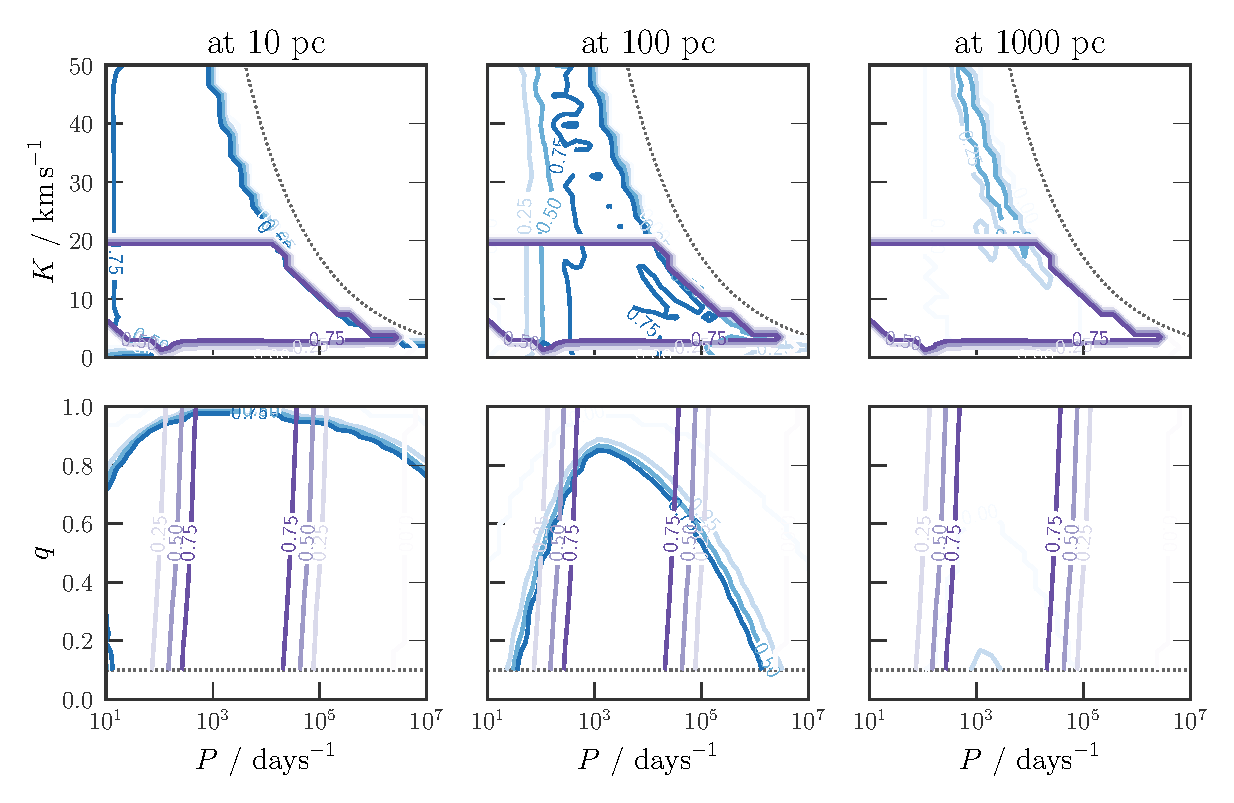
\includegraphics[width=\textwidth]{detection_efficiency_ms_ms_binaries.pdf}
    \caption{}
    \label{fig:detection-efficiency-ms-ms-binaries}
\end{figure}











\section{Results} \label{sec:results}




We confirm that most stars are in binaries or higher order multiples.
A cross-match of our catalog with the ninth spectroscopic binary catalog
\citep{SB9} reveals that we confidently detect SB1-type binary systems (from
radial velocity variations) with semi-amplitudes down to $K \approx \todo{X}\,\textrm{km\,s}^{-1}$ and orbital
periods as long as about 44\,months ($\approx3.5$\,yr) -- twice the observing span
of the second \Gaia\ data release. Both of these bounds are expected: at low $K$ \Gaia\
lacks the radial velocity precision to distinguish single stars from stellar multiples,
and only half the orbital period is required to accurately estimate the peak-to-peak radial velocity variations.
If the orbital period is longer, we can still reliably identify some systems as stellar
multiples if the radial velocity semi-amplitude is large enough, but in these instances we will
systematically underestimate the true radial velocity semi-amplitude because \Gaia\ has not
observed at least half the orbital period and we do not have access to the radial velocity
measurements at each epoch to fit a Keplerian curve. In other words, we implicitly assume
that \Gaia\ has observed at least half the orbital period for every binary system we detect.
If this assumption is not met, our radial velocity semi-amplitude estimates will be underestimated
by about the same fraction of the observing span relative to half the true orbital period.

We accurately estimate the radial velocity semi-amplitude for well-studied SB1-type systems
with periods $P < 44\,\textrm{months}$ (Figure \ref{fig:rv-sb9-comparison}). \todo{Our estimated
errors on $K$ also appear reasonably consistent given more precise literature estimates.}
The estimates of $K$ and their associated errors could be improved by considering the exact
moments when \Gaia\ observed each source -- even if the actual measurement at each epoch is
not known -- but we consider that to be a useful extension of this work. \todo{In Figure \ref{fig:rv-p-k}
we show the orbital periods and radial velocity semi-amplitudes where we confidently detect binary
systems.}




\begin{figure}
	\centering
	%\includegraphics[width=0.5\textwidth]{scatter-excess-rv-jitter-for-known-binaries-sb9.png}
    \caption{Estimated orbital semi-amplitude $K_\textrm{est}$ from excess radial velocity jitter in
    		 \Gaia\ compared with estimates from long-term radial velocity measurements as reported
    		 by the ninth spectroscopic binary catalog \citep{Pourbaix:2004}.
    		 % TODO: [ ] Points coloured by what.
    		 % 		 [ ] What restrictions did we do for this sample?
    		 % 	     [ ] Minimum reliably detectable K_est?
    		}
    \label{fig:sb9-compare-rv-semi-amplitude}
\end{figure}






\todo{Comparison with APW unimodal; APW first percentile}

\todo{Comparison with astrometric binaries detected -- are there any catalogs of these?}

\todo{Comparison with Badenes, Troup}

\todo{Comparison with Ragahvan, who had many different detection methods}

\subsection{Stellar multiplicity across the Hertszprung-Russell diagram}


\subsection{The stellar multiplicity fraction}

\todo{Binary fraction as a function of everything}



\begin{figure}
	\centering
	%\includegraphics[width=0.5\textwidth]{scatter-period-and-rv-semiamplitude-for-known-binaries-all.png}
    \caption{Orbital period and radial velocity semi-amplitude for known binary systems
    		 \citep{Pourbaix:2004, APW, Others}. Points are coloured by our estimated probability of
    		 being a single star, given the \Gaia\ radial velocity jitter. The dashed line indicates
    		 the observing span of \Gaia\ DR2, and the solid line shows twice the observing span.
    		 Qualitatively it is clear that we can detect binaries with orbital periods nearly twice
    		 the observing span if the radial velocity semi-amplitude is large enough.}
    \label{fig:PK-all-known-binaries}
\end{figure}




\section{Discussion} \label{sec:discussion}

\begin{itemize}
	\item {Binary fraction in the spaces that we were fitting: rp flux, colour, etc, just showing the transition of probabilities}
	\item {Binary fraction as a function of fitting properties (e.g., colour, absolute RP mag, apparent RP mag)}
	\item {Binarity across the H-R diagram}
	\item {What are the distributions of orbital parameters of binary systems that we would be able to detect?}
	\item {Binarity with respect to metallicity}
    \item {Binarity in clusters vs the field?}
    \item {Binarity among extremely metal-poor stars?}
    \item {Superlative systems (\eg, stellar mass black-hole companions)}
\end{itemize}


\section{Conclusions} \label{sec:conclusions}
See abstract.


\acknowledgements

% At least some of these people will be promoted to the author list.
It is a pleasure to thank
	Berry Holl (Observatoire de Gen\'eve),
	Jose Hernandez (ESAC),
	Daniel Michalik (ESA/ESTEC),
	Kevin C. Schlaufman (Johns Hopkins University),
	Lorenzo Spina (Monash University),
		and
	Sergey Koposov (Carnegie Mellon University).

This research was developed in part at 
	the NYC Gaia DR2 Workshop at the Center for Computational Astrophysics of the Flatiron Institute 
		in 2018 April, and at
	the 2019 Santa Barbara Gaia Sprint, hosted by the Kavli Institute for Theoretical Physics at the 
		University of California, Santa Barbara

A.~R.~C. is supported in part by the Australian Research Council through a Discovery Early Career 
Researcher Award (DE190100656). 
Parts of this research were supported by the Australian Research Council Centre of Excellence for 
All Sky Astrophysics in 3 Dimensions (ASTRO 3D), through project number CE170100013.
This research was supported in part at KITP by the Heising-Simons Foundation and the National 
Science Foundation under Grant No. NSF PHY-1748958.

This work has made use of data from the European Space Agency (ESA) mission {\it
Gaia} (\url{https://www.cosmos.esa.int/gaia}), processed by the {\it Gaia} Data
Processing and Analysis Consortium (DPAC,
\url{https://www.cosmos.esa.int/web/gaia/dpac/consortium}). Funding for the DPAC
has been provided by national institutions, in particular the institutions
participating in the {\it Gaia} Multilateral Agreement.  

This work has made use of CosmoHub. CosmoHub has been developed by the Port 
d'Informaci\'o Cient\'ifica (PIC), maintained through a collaboration of the 
Institut de F\'isica d'Altes Energies (IFAE) and the Centro de Investigaciones 
Energ\'eticas, Medioambientales y Tecnol\'ogicas (CIEMAT), and was partially 
funded by the ``Plan Estatal de Investigaci\'on Cient�fica y T\'ecnica y de 
Innovaci\'on'' program of the Spanish government.

\software{
	\package{Astropy} \citep{astropy:2013,astropy:2018},
    \package{IPython} \citep{ipython},
    \package{matplotlib} \citep{mpl},
    \package{numpy} \citep{numpy},
    \package{scipy} \citep{scipy},
    \package{Stan} \citep{stan},
    \package{CosmoHub} \citep{Carretero:2017},
    \package{TensorFlow} \citep{tensorflow}
    \package{Jupyter Notebooks} \citep{jupyter-notebooks}
}    


\appendix

\section{Reproducibility} \label{app:reproducibility}

This project was developed in a \texttt{git} repository hosted at \giturl. 
The repository includes notebooks that demonstrate the progression our work,  
\LaTeX\ to compile this manuscript, and scripts to reproduce the analysis described
in this manuscript. 
We executed the following
Astronomical Data Query Language (\texttt{ADQL})\footnote{http://www.ivoa.net/documents/latest/ADQL.html} 
query through CosmoHub \citep{Carretero:2017} to retrieve the \Gaia\ data:
\begin{comment}
\begin{minted}[style=friendly]{postgresql}
 SELECT *
   FROM gaiadr2.gaia_source
  WHERE phot_g_mean_mag <= 14
\end{minted}
\end{comment}

The results presented here can be reproduced in full (including data
retrieval, analysis, creation of figures, and manuscript compilation) using these
commands in a modern terminal:
% this is not python, but latex fails to evaluate \githash if I set bash environment.
\begin{comment}
\begin{minted}[
style=friendly,
escapeinside=||
]{python} 
git clone https://github.com/andycasey/velociraptor.git velociraptor
cd velociraptor
git checkout |\githash|
./reproduce
\end{minted}
\end{comment}

Reproducing these results will require at least \todo{X}\,Gb of free disk space 
and \todo{Y}\,hours of compute time. The settings in the \texttt{model.yml} file
can be adjusted to reduce the sample size of the data and shorten the compute 
time at the expense of accuracy. 



\section{Proof of {$K = \sqrt{2}\RVJitter$} for well-sampled circular orbits} \label{app:prove-K}

This proof is not new. 
It is included here as a refresher. 
Consider a binary system on a circular orbit. 
The radial velocity of the system at any time $t$ is given by
\begin{eqnarray}
	v_r(t) = \gamma + K\sin\left(\frac{2\pi}{P}t + \varphi_0\right)
\end{eqnarray}
\noindent{}where $\gamma$ is the systemic radial velocity, $P$ is the orbital period, $\varphi_0$ is the phase of the initial observation at $t_0$, and $K$ is the radial velocity semi-amplitude. 
Let $\omega = \frac{2\pi}{P}$. 
If the observed baseline $T > \frac{P}{2}$ and $t \sim \mathcal{U}\left(0,T\right)$ then we can ignore the initial phase $\varphi_0$.

The root mean square for a continuous function over some time interval $T$ is
\begin{eqnarray}
v_\mathrm{rms}^2 &=& \frac{1}{T}\int_{0}^{T}\left[v_r(t)\right]^2 \partial{}t \\
v_\mathrm{rms}^2 &=& \frac{1}{T}\int_{0}^{T}\left[\gamma + K\sin(\omega{}t)\right]^2\partial{}t\\
v_\mathrm{rms}^2 &=& \frac{1}{T}\int_{0}^{T}\left[\gamma^2 + 2K\gamma\sin\left(\omega{}t\right) + K^2\sin^2\left(\omega{}t\right)\right] \partial{}t
% By making use of the double-angle formulae
%v_\mathrm{rms}^2 &=& \frac{1}{T}\left[\gamma^2{t}|_0^{T} + \frac{2K\gamma}{\omega}\cos{\left(\omega{}t\right)}|_0^T + \frac{K^2}{2}\int_0^T\left(1 - \cos\left(2\omega{}t\right)\right)\partial{}t\right]
\end{eqnarray}


After expanding terms and using the identity
\begin{eqnarray}
	\sin^2\left(\omega{}t\right) = \frac{1}{2}\left[1 - \cos\left(2\omega{}t\right)\right]
\end{eqnarray}
\noindent{}we find \todo{Fill in from notebook}


\noindent{}giving 
\begin{eqnarray}
	K = \sqrt{2}\RVJitter \quad .
\end{eqnarray}


If we assume that each radial velocity measurement has some associated noise, and that noise is
homoskedastic, then an unbiased estimate of the radial velocity semi-amplitude is given by
\begin{eqnarray}
	\todo{K = }
\end{eqnarray}
\noindent{}and the error on that estimate is \todo{T.~B.~C.}


\section{Radial velocity completeness as a function of \Gaia\ source properties} \label{app:missing-rvs}

Many sources in the second \Gaia\ data release do not have a reported radial 
velocity, despite being bright enough ($G \lesssim 13$) and in a suitable 
temperature range (e.g., between $\approx4000\,\textrm{K}$ and $\approx6500\,\textrm{K}$) 
for radial velocities to be measured \citep{Cropper:2018}. One reason 
why radial velocity measurements are \emph{not} reported for these stars is 
because the \Gaia/DPAC team have may identified the source to be a double-lined 
spectroscopic binary (a so-called SB2-type system), either through a 
composition of two stellar sources present in the spectra, or from multiple 
(significant) modes in the cross-correlation function. In these situations it
is not sensible to report a point estimate of the radial velocity of the point 
source. 

Another likely explanation is that the system is a binary system with a large
radial velocity semi-amplitude (e.g., a main-sequence binary pair), leading to
a radial velocity error $\sigma_{\textrm{V}_\textrm{R}}^\textrm{MTA}$ exceeding 20\,km\,s$^{-1}$ 
(irrespective of the number of transits). In these cases the radial velocity for that source would be removed because the \Gaia/DPAC team
decided that sources with radial velocity errors exceeding 20\,km\,s$^{-1}$ are likely spurious
(e.g., due to source confusion). Although this is a judicious decision, it has the consequence of removing
the radial velocity \emph{and} the radial velocity error for many main-sequence binary pairs,
and systems with non-luminous companions (e.g., black holes, neutron stars).
As we have shown, even if the radial velocity were removed, the radial velocity \emph{error}
can be used to infer properties about binary systems.


This motivated us to investigate whether a \emph{lack} radial velocity was indicative of stellar multiplicity. 
We advise against this.
We calculated the completeness of radial velocity measurements (e.g., the
fraction of sources with reported radial velocities) as a function of all 
available source properties that might affect whether the radial velocity may
be reported or not. This included position ($\alpha$, $\delta$, $l$, $b$),
parallax, proper motions, apparent magnitudes, $\Gbp\ - \Grp$ colour, 
properties of the radial velocity templates, stellar parameters ($\teff$, $\radius$, $\luminosity$),
and other properties. 

We took all sources with \todo{$\Grp < 12$ and $0.YY \geq \Gbp\ - \Grp \geq 0.XX$}, where the
fraction of sources with radial velocity measurements in this sample is relatively flat with respect
to colour and apparent magnitude.
However, when the density of sources is shown as a function of sky position (Figure~\ref{fig:missing-rvs-sky-location})
it is clear that the presence (or absence) of radial velocity measurements is strongly dependent on
sky position.
%Some of this is attributable to a higher likelihood of source confusion in the Milky Way disk, but
%not all
The sky pattern observed is an function of 
	the initial \Gaia\ source catalog list \citep{Someone},
	the scanning law (\ie, some parts of the sky are observed less frequently), and
	higher likelihood of source confusion in dense regions (\eg, the Milky Way disk and bulge).
For these reasons, we conclude that the \emph{lack} of radial velocity information is not
informative of binarity.\footnote{The astute reader might remark `Duh!', but numerous groups have
	sought to use the lack of radial velocity information as informative of binarity
	(or low metallicity) before they also came to this conclusion.}

% This is illustrated in Appendix~\ref{app:missing-rvs}, where we show that an absence of radial
%velocity is a combination of sky completeness, the initial \Gaia\ source
%catalog, as well as stellar multiplicity. For these reasons, if a \Gaia\
%source does not have a radial velocity error then we only use the astrometric
%jitter to inform us about stellar multiplicity.



\begin{figure*}
%	%%\includegraphics[width=1.0\textwidth]{../figures/sb2_rvs_completeness.pdf}
%	%%\includegraphics[width=1.0\textwidth]{../figures/todo.png}
    \caption{Fraction of \Gaia\ sources with reported radial velocities
		     as a function of source properties. Within the adopted source
		     parameter ranges (gray; see Section \ref{sec:sb2_methods})
		     the radial velocity completeness is approximately flat.
		     We flag sources within this range that do not have reported 
		     radial velocities to be candidate SB2 systems.}
    \label{fig:sb2_rvs_completeness}
\end{figure*}




\begin{figure*}
%	%%\includegraphics[width=1.0\textwidth]{../figures/sb2_sky_structure.pdf}
%	%%\includegraphics[width=1.0\textwidth]{../figures/todo.png}
    \caption{Fraction of sources (per sky bin) without reported radial velocities
    		 for all sources with $G \lesssim 13$ (top) and sources in the ranges
		 	 specified by Eqs \ref{eq:sb2_ranges} (bottom), where we assert that a missing
			 radial velocity measurement signifies a likely SB2 candidate . The color scale is 
			 arbitrarily set to highlight structure, where black indicates a higher
			 fraction of sources do not have reported radial velocities. Crowding
			 in the galactic plane likely results in some sources not having radial
			 velocities reported. The large scale structure visible in both axes is
			 a combined effect of the initial \Gaia\ source list, the scanning law,
			 and star forming regions (i.e., where emission in the \ion{Ca}{2} 
			 triplet likely causes issues for radial velocity determination).}
    \label{fig:sb2_sky_structure}
\end{figure*}





\bibliography{trex}{}
\bibliographystyle{aasjournal}

%\listofchanges

\end{document}
